
\newpage

\subsection{Numerical Analysis}

Numerical analysis is an area of mathematics and computer science that
creates, analyzes, and implements algorithms for approximating
numerical solutions to problems involving continuous variables
\cite{brezinski2012numerical}. For simplicity, a specific kind of
annulus is considered, which has the radius ratio $\mu=2$. 

The preliminary step of the evaluation of $S(\tau)$, a general
Dirichlet series, and $\langle \tau \rangle$ is to compute the
monotonically increasing $\lambda_{0,n}$ of Eq.$(2.7)$. The $n$th
positive zero $\lambda_{0,n}$, as $n \rightarrow \infty $, can be
bracketed in an interval $((n-1) \pi, (n+1) \pi)$
\cite{NIST:DLMF}. Bisection method \cite{2020SciPy-NMeth}, a
well-known and most reliable root finding method. It can be used to
close in on the root by successivly halving the interval until it
becomes sufficiently small.

\begin{figure}[h!]
  \centering
  \subfloat[]{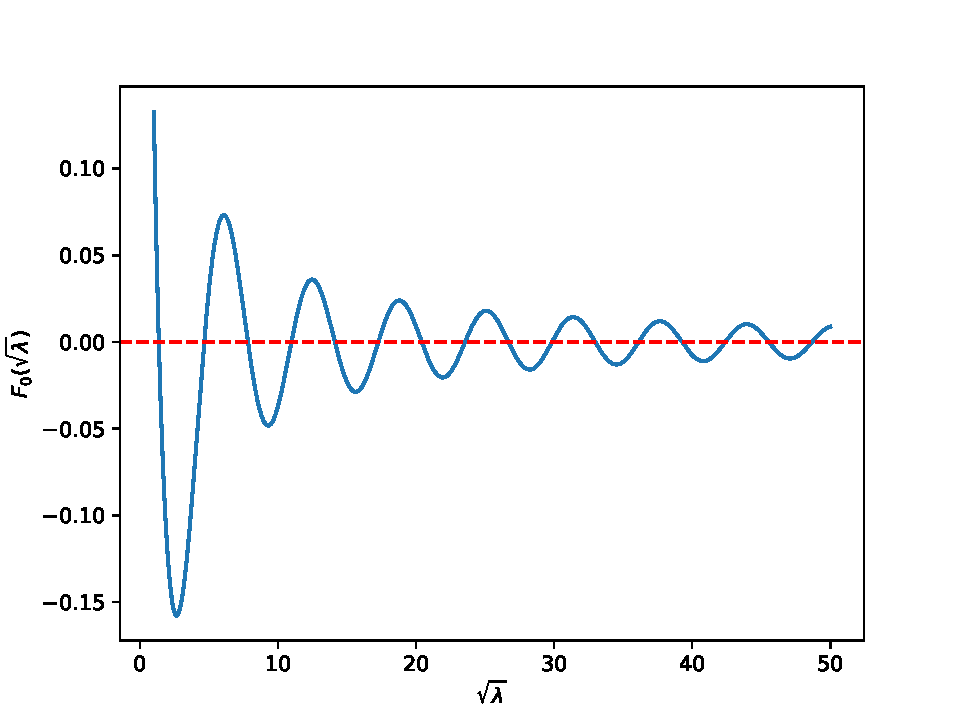
\includegraphics[width=0.5\textwidth]{F0}}%
  %\qquad
  \subfloat[]{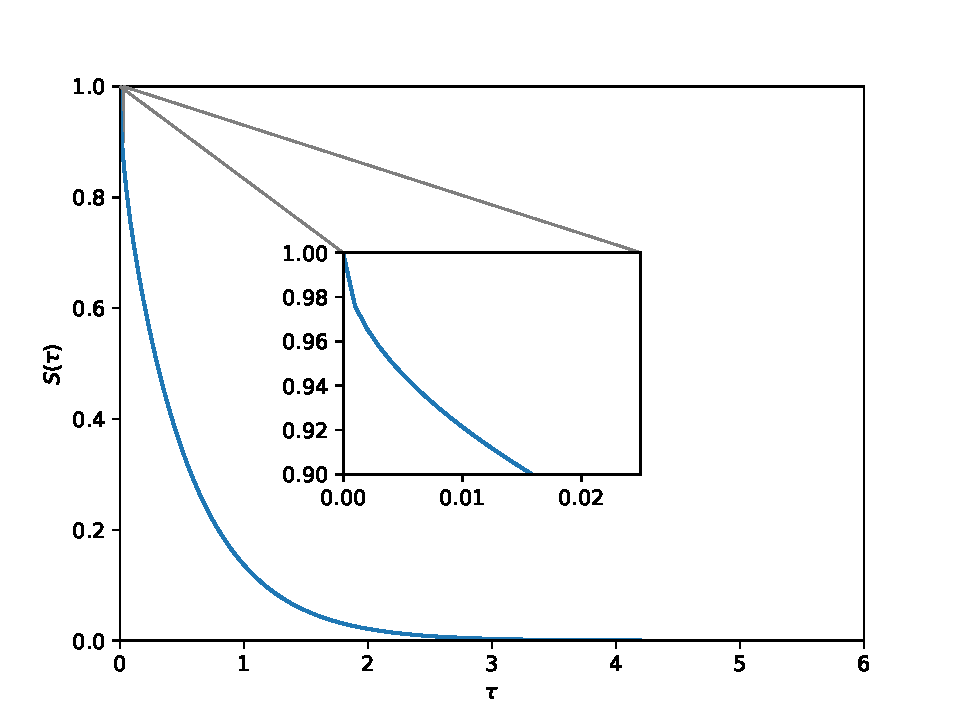
\includegraphics[width=0.5\textwidth]{analytical_s}}%
  \caption{(a) It is straightforward to evaluate the cross-product of
    Bessel fucntions by SciPy library \cite{2020SciPy-NMeth}. (b) The
    asymptotic behaviors of survival probability $S(\tau)$ are
    approximated by the numerical method with the first $1000$
    eigenvalues. $S(\tau)$ monotonously descrese from 1 at $\tau=0$ to
    $0$ as $\tau$ goes to infinity. Moreover, the approximation of
    analytical mean first-passage time $\langle \tau \rangle$ equals
    $0.47339248$.}
\end{figure}




